\begin{tikzpicture}[scale=0.52]
	\begin{axis} [
		title = {\LARGE $\Hbarc[\field]{m}{\VS},\, u_m\neq 0$},
		ticklabel style = {font=\Large},
		axis y line=middle,
		axis x line=middle,
		ytick={0.5,0.6,0.67,0.95},
		yticklabels={,$ \zeta_m$,,$\pi$},
		xtick={0.5,0.55,0.95},
		xticklabels={ ,$\zeta_n$, $\pi$},
		xmin=-0.015, xmax=1.1,
		ymin=0, ymax=1.1,]
		\addplot [mark=none] coordinates {(0,0) (1,1)};
		\addplot [thick,color=black!20!white,fill=black!30!white,
		fill opacity=0.4]coordinates {
			(0.55,0.95)
			(0.55,0.55)
			(0.95,0.95)
			(0.55,0.95)};
		\addplot [black!40!white,mark=none,dashed, thin] coordinates {(0,0.6) (0.6,0.6)};
		\addplot [black!40!white,mark=none,dashed, thin] coordinates {(0,0.55) (0.55,0.55)};
		\addplot [black!40!white,mark=none,dashed, thin] coordinates {(0.55,0) (0.55,0.55)};
		\addplot[barccolor,mark=*] (0, 0.6) circle (2pt) node[above right,barccolor]{};%{\Large\textsf{1}};
		%\node[mark=none] at (axis cs:0.68,0.21){$\Hbarc{2}{\VS^n}$};
	\end{axis}
\end{tikzpicture}
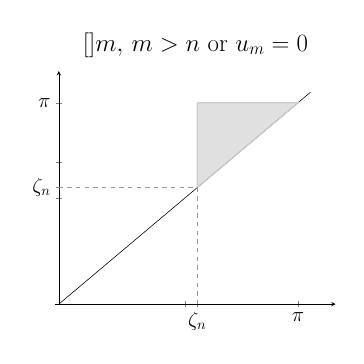
\begin{tikzpicture}[scale=0.52]
	\begin{axis} [
		title = {\LARGE $\Hbarc[\field]{m}{\VS},\, m>n$ or $u_m = 0$},
		ticklabel style = {font=\Large},
		axis y line=middle,
		axis x line=middle,
		ytick={0.5,0.55,0.67,0.95},
		yticklabels={,$\zeta_n$,,$\pi$},
		xtick={0.5,0.55,0.95},
		xticklabels={ ,$\zeta_n$, $\pi$},
		xmin=-0.015, xmax=1.1,
		ymin=0, ymax=1.1,]
		\addplot [mark=none] coordinates {(0,0) (1,1)};
		\addplot [thick,color=black!20!white,fill=black!30!white,
		fill opacity=0.4]coordinates {
			(0.55,0.95)
			(0.55,0.55)
			(0.95,0.95)
			(0.55,0.95)};
		\addplot [black!40!white,mark=none,dashed, thin] coordinates {(0,0.55) (0.55,0.55)};
		\addplot [black!40!white,mark=none,dashed, thin] coordinates {(0.55,0) (0.55,0.55)};
		%\node[mark=none] at (axis cs:0.68,0.21){$\Hbarc[\field]{m}{\VS^n}, m\geq 3$};
	\end{axis}
\end{tikzpicture}

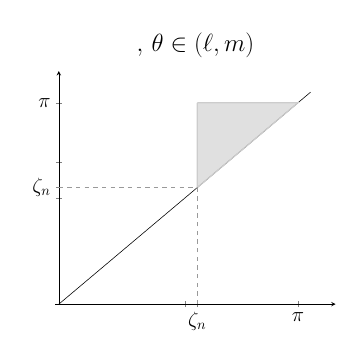
\begin{tikzpicture}[scale=0.52]
	\begin{axis} [
		title={\LARGE $\thetabarc{\VS},\, \theta \in \cO(\ell,m)$},
		ticklabel style = {font=\Large},
		axis y line=middle,
		axis x line=middle,
		ytick={0.5,0.55,0.67,0.95},
		yticklabels={,$\zeta_n$,,$\pi$},
		xtick={0.5,0.55,0.95},
		xticklabels={ ,$\zeta_n$, $\pi$},
		xmin=-0.015, xmax=1.1,
		ymin=0, ymax=1.1,]
		\addplot [mark=none] coordinates {(0,0) (1,1)};
		\addplot [thick,color=black!20!white,fill=black!30!white,
		fill opacity=0.4]coordinates {
			(0.55,0.95)
			(0.55,0.55)
			(0.95,0.95)
			(0.55,0.95)};
		\addplot [black!40!white,mark=none,dashed, thin] coordinates {(0,0.55) (0.55,0.55)};
		\addplot [black!40!white,mark=none,dashed, thin] coordinates {(0.55,0) (0.55,0.55)};
		%\node[mark=none] at (axis cs:0.68,0.21){$\sqbarc{k}{\VS^n},\, k\geq 1$};
	\end{axis}
\end{tikzpicture}
